\documentclass{standalone}
\usepackage{tikz}
\usetikzlibrary{patterns, positioning}


\begin{document}
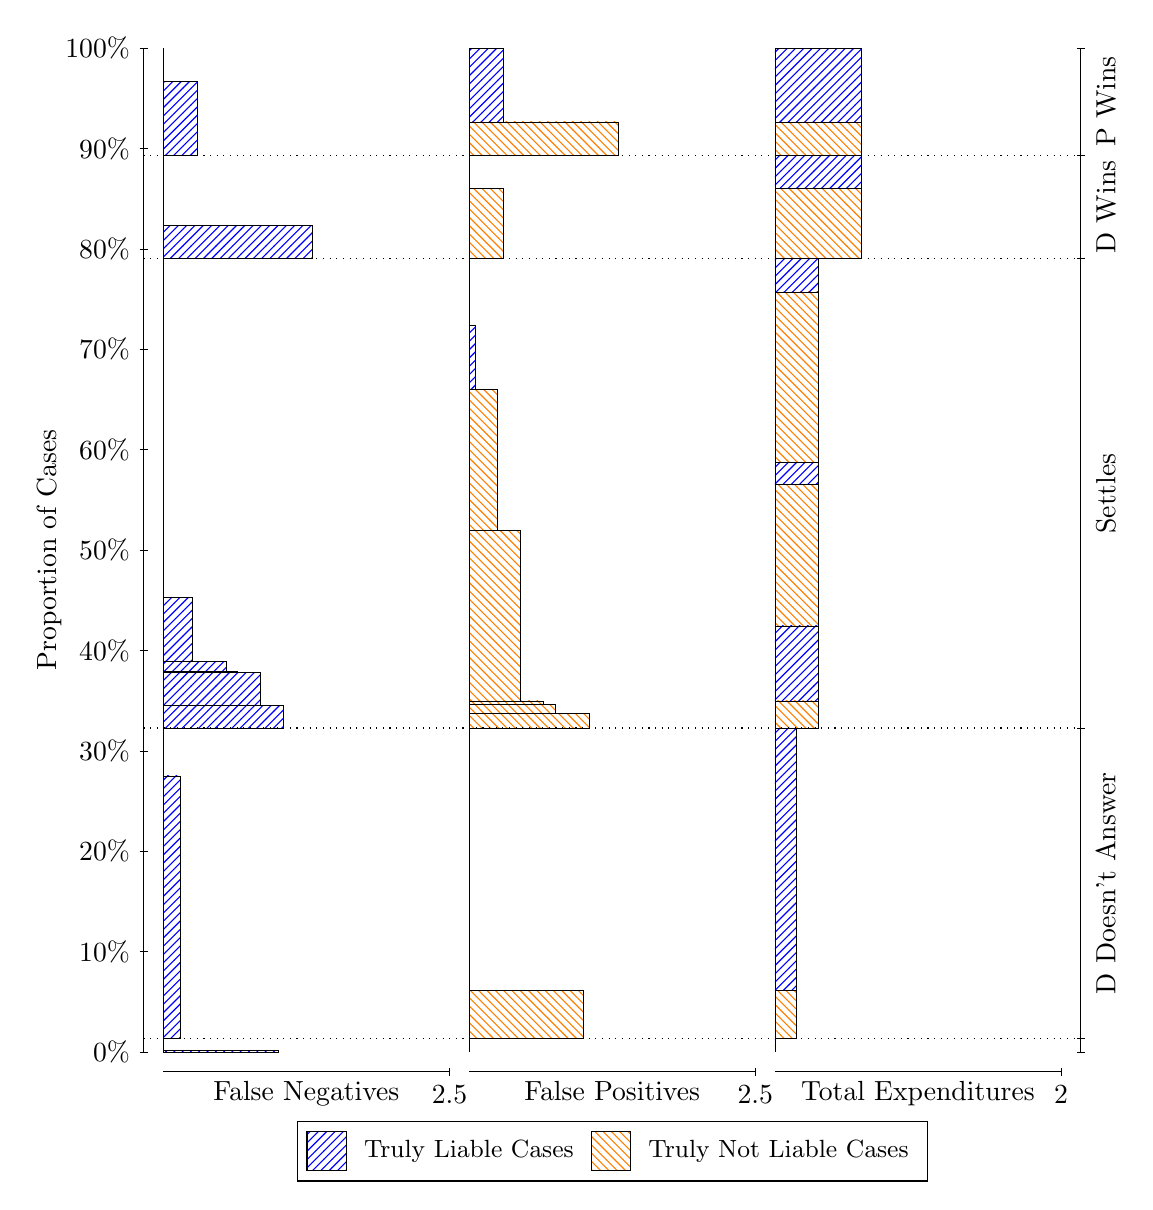
\begin{tikzpicture}
\draw[black, very thin] (1.5,1.75) -- (1.5,14.5);
\node[rotate=90, text=black, anchor=center] at (0.3, 8.125) {Proportion of Cases};
\draw[black, very thin] (1.45,1.75) -- (1.55,1.75);
\node[text=black, anchor=east] at (1.45, 1.75) {0\%};
\draw[black, very thin] (1.45,3.025) -- (1.55,3.025);
\node[text=black, anchor=east] at (1.45, 3.025) {10\%};
\draw[black, very thin] (1.45,4.3) -- (1.55,4.3);
\node[text=black, anchor=east] at (1.45, 4.3) {20\%};
\draw[black, very thin] (1.45,5.575) -- (1.55,5.575);
\node[text=black, anchor=east] at (1.45, 5.575) {30\%};
\draw[black, very thin] (1.45,6.85) -- (1.55,6.85);
\node[text=black, anchor=east] at (1.45, 6.85) {40\%};
\draw[black, very thin] (1.45,8.125) -- (1.55,8.125);
\node[text=black, anchor=east] at (1.45, 8.125) {50\%};
\draw[black, very thin] (1.45,9.4) -- (1.55,9.4);
\node[text=black, anchor=east] at (1.45, 9.4) {60\%};
\draw[black, very thin] (1.45,10.675) -- (1.55,10.675);
\node[text=black, anchor=east] at (1.45, 10.675) {70\%};
\draw[black, very thin] (1.45,11.95) -- (1.55,11.95);
\node[text=black, anchor=east] at (1.45, 11.95) {80\%};
\draw[black, very thin] (1.45,13.225) -- (1.55,13.225);
\node[text=black, anchor=east] at (1.45, 13.225) {90\%};
\draw[black, very thin] (1.45,14.5) -- (1.55,14.5);
\node[text=black, anchor=east] at (1.45, 14.5) {100\%};

\draw[black, very thin] (13.4,1.75) -- (13.4,14.5);
\draw[black, very thin] (13.35,1.75) -- (13.45,1.75);
\node[anchor=west] at (13.35, 1.75) {};
\draw[black, very thin] (13.35,1.9185) -- (13.45,1.9185);
\node[anchor=west] at (13.35, 1.9185) {};
\draw[black, very thin] (13.35,5.8644) -- (13.45,5.8644);
\node[anchor=west] at (13.35, 5.8644) {};
\draw[black, very thin] (13.35,11.824) -- (13.45,11.824);
\node[anchor=west] at (13.35, 11.824) {};
\draw[black, very thin] (13.35,13.138) -- (13.45,13.138);
\node[anchor=west] at (13.35, 13.138) {};
\draw[black, very thin] (13.35,14.5) -- (13.45,14.5);
\node[anchor=west] at (13.35, 14.5) {};

\draw[black, very thin, pattern color=blue, pattern=north east lines] (1.75,1.75) rectangle (3.2033,1.7677);
\draw[black, very thin, pattern color=orange, pattern=north west lines] (1.75,1.7677) rectangle (1.75,1.9185);
\draw[black, very thin, pattern color=blue, pattern=north east lines] (1.75,1.9185) rectangle (1.968,5.2551);
\draw[black, very thin, pattern color=orange, pattern=north west lines] (1.75,5.2551) rectangle (1.75,5.8644);
\draw[black, very thin, pattern color=blue, pattern=north east lines] (1.75,5.8644) rectangle (3.276,6.1511);
\draw[black, very thin, pattern color=blue, pattern=north east lines] (1.75,6.1511) rectangle (2.9853,6.5703);
\draw[black, very thin, pattern color=blue, pattern=north east lines] (1.75,6.5703) rectangle (2.6947,6.5863);
\draw[black, very thin, pattern color=blue, pattern=north east lines] (1.75,6.5863) rectangle (2.5493,6.7137);
\draw[black, very thin, pattern color=blue, pattern=north east lines] (1.75,6.7137) rectangle (2.1133,7.523);
\draw[black, very thin, pattern color=orange, pattern=north west lines] (1.75,7.523) rectangle (1.75,11.824);
\draw[black, very thin, pattern color=blue, pattern=north east lines] (1.75,11.824) rectangle (3.6393,12.246);
\draw[black, very thin, pattern color=orange, pattern=north west lines] (1.75,12.246) rectangle (1.75,13.138);
\draw[black, very thin, pattern color=blue, pattern=north east lines] (1.75,13.138) rectangle (2.186,14.077);
\draw[black, very thin, pattern color=orange, pattern=north west lines] (1.75,14.077) rectangle (1.75,14.5);
\draw[black, very thin, pattern color=orange, pattern=north west lines] (5.6333,1.75) rectangle (5.6333,1.9008);
\draw[black, very thin, pattern color=blue, pattern=north east lines] (5.6333,1.9008) rectangle (5.6333,1.9185);
\draw[black, very thin, pattern color=orange, pattern=north west lines] (5.6333,1.9185) rectangle (7.0867,2.5279);
\draw[black, very thin, pattern color=blue, pattern=north east lines] (5.6333,2.5279) rectangle (5.6333,5.8644);
\draw[black, very thin, pattern color=orange, pattern=north west lines] (5.6333,5.8644) rectangle (7.1593,6.0539);
\draw[black, very thin, pattern color=orange, pattern=north west lines] (5.6333,6.0539) rectangle (6.7233,6.164);
\draw[black, very thin, pattern color=orange, pattern=north west lines] (5.6333,6.164) rectangle (6.578,6.2084);
\draw[black, very thin, pattern color=orange, pattern=north west lines] (5.6333,6.2084) rectangle (6.2873,8.3717);
\draw[black, very thin, pattern color=orange, pattern=north west lines] (5.6333,8.3717) rectangle (5.9967,10.165);
\draw[black, very thin, pattern color=blue, pattern=north east lines] (5.6333,10.165) rectangle (5.706,10.975);
\draw[black, very thin, pattern color=blue, pattern=north east lines] (5.6333,10.975) rectangle (5.6333,11.824);
\draw[black, very thin, pattern color=orange, pattern=north west lines] (5.6333,11.824) rectangle (6.0693,12.715);
\draw[black, very thin, pattern color=blue, pattern=north east lines] (5.6333,12.715) rectangle (5.6333,13.138);
\draw[black, very thin, pattern color=orange, pattern=north west lines] (5.6333,13.138) rectangle (7.5227,13.561);
\draw[black, very thin, pattern color=blue, pattern=north east lines] (5.6333,13.561) rectangle (6.0693,14.5);
\draw[black, very thin, pattern color=orange, pattern=north west lines] (9.5167,1.75) rectangle (9.5167,1.9008);
\draw[black, very thin, pattern color=blue, pattern=north east lines] (9.5167,1.9008) rectangle (9.5167,1.9185);
\draw[black, very thin, pattern color=orange, pattern=north west lines] (9.5167,1.9185) rectangle (9.7892,2.5279);
\draw[black, very thin, pattern color=blue, pattern=north east lines] (9.5167,2.5279) rectangle (9.7892,5.8644);
\draw[black, very thin, pattern color=orange, pattern=north west lines] (9.5167,5.8644) rectangle (10.062,6.2084);
\draw[black, very thin, pattern color=blue, pattern=north east lines] (9.5167,6.2084) rectangle (10.062,7.1611);
\draw[black, very thin, pattern color=orange, pattern=north west lines] (9.5167,7.1611) rectangle (10.062,8.9545);
\draw[black, very thin, pattern color=blue, pattern=north east lines] (9.5167,8.9545) rectangle (10.062,9.2411);
\draw[black, very thin, pattern color=orange, pattern=north west lines] (9.5167,9.2411) rectangle (10.062,11.404);
\draw[black, very thin, pattern color=blue, pattern=north east lines] (9.5167,11.404) rectangle (10.062,11.824);
\draw[black, very thin, pattern color=orange, pattern=north west lines] (9.5167,11.824) rectangle (10.607,12.715);
\draw[black, very thin, pattern color=blue, pattern=north east lines] (9.5167,12.715) rectangle (10.607,13.138);
\draw[black, very thin, pattern color=orange, pattern=north west lines] (9.5167,13.138) rectangle (10.607,13.561);
\draw[black, very thin, pattern color=blue, pattern=north east lines] (9.5167,13.561) rectangle (10.607,14.5);
\draw[black, dotted] (1.5,1.9185) -- (13.4,1.9185);
\draw[black, dotted] (1.5,5.8644) -- (13.4,5.8644);
\draw[black, dotted] (1.5,11.824) -- (13.4,11.824);
\draw[black, dotted] (1.5,13.138) -- (13.4,13.138);
\draw[black, very thin] (1.75,1.5) -- (5.3833,1.5);
\node[text=black, anchor=north] at (3.5667, 1.5) {False Negatives};
\draw[black, very thin] (5.3833,1.45) -- (5.3833,1.55);
\node[text=black, anchor=north] at (5.3833, 1.45) {2.5};

\draw[black, very thin] (5.6333,1.5) -- (9.2667,1.5);
\node[text=black, anchor=north] at (7.45, 1.5) {False Positives};
\draw[black, very thin] (9.2667,1.45) -- (9.2667,1.55);
\node[text=black, anchor=north] at (9.2667, 1.45) {2.5};

\draw[black, very thin] (9.5167,1.5) -- (13.15,1.5);
\node[text=black, anchor=north] at (11.333, 1.5) {Total Expenditures};
\draw[black, very thin] (13.15,1.45) -- (13.15,1.55);
\node[text=black, anchor=north] at (13.15, 1.45) {2};


\node[text=black, centered, rotate=90] at (13.72, 3.8915) {D Doesn't Answer};
\node[text=black, centered, rotate=90] at (13.72, 8.8441) {Settles};
\node[text=black, centered, rotate=90] at (13.72, 12.481) {D Wins};
\node[text=black, centered, rotate=90] at (13.72, 13.819) {P Wins};

\draw (7.449999999999999,1.5) node[draw=none] (baseCoordinate) {};
\begin{scope}[align=center]
        \matrix[scale=0.5, draw=black, below=0.5cm of baseCoordinate, nodes={draw}, column sep=0.1cm]{
            \node[rectangle, draw, minimum width=0.5cm, minimum height=0.5cm, pattern color=blue, pattern=north east lines] {}; &
            \node[draw=none, font=\small, text=black] (B) {Truly Liable Cases}; &
            \node[rectangle, draw, minimum width=0.5cm, minimum height=0.5cm, pattern color=orange, pattern=north west lines] {}; &
            \node[draw=none, font=\small, text=black] (B) {Truly Not Liable Cases}; \\
            };
\end{scope}

\end{tikzpicture}
\end{document}